\documentclass[10pt]{beamer}
% \setbeameroption{show only notes}

\usetheme[progressbar=foot]{metropolis}
\makeatletter
\usepackage[caption=false]{subfig}
\usepackage{float}
\usepackage{textgreek}
\usepackage{amsmath}
\newlength\beamerleftmargin
\setlength\beamerleftmargin{\Gm@lmargin}
\usepackage[absolute,overlay]{textpos}
\usepackage{appendixnumberbeamer}
\setbeamertemplate{section in toc}[sections numbered]
\setbeamertemplate{subsection in toc}[subsections numbered]
\usepackage{booktabs}
\usepackage[scale=2]{ccicons}
\definecolor{utred}{RGB}{204,0,0}
\definecolor{utgray}{RGB}{128,128,128}
\usepackage{tikz}
\usepackage{graphicx}
\usepackage{pgfplots}
\usepackage{caption}
\newcommand{\vect}[1]{\boldsymbol{#1}}
\newcommand{\tn}{\textnormal}

\graphicspath{{/Users/andrewwork/thesis/reg_stokeslets/plots/}}

\captionsetup[figure]{labelformat=empty}
\setbeamertemplate{subsectionin toc}
{\leavevmode\leftskip=2em
  \rlap{
    \hskip-2em$\quad$\inserttocsectionnumber.\inserttocsubsectionnumber
  }
  $\quad$\inserttocsubsection\par}
%%%%%%
\usepgfplotslibrary{dateplot}

\usepackage{xspace}
\newcommand{\themename}{\textbf{\textsc{metropolis}}\xspace}

\title{Platelet Rolling: Pole Vaulting and Surfing}
\date{\today}
\author{Andrew Watson}
\institute{University of Utah}
% \titlegraphic{\hfill\includegraphics[height=1.5cm]{logo.pdf}}

\setbeamercolor{progress bar in head/foot}{fg=utred,bg=utgray}
\setbeamercolor{progress bar in section page}{fg=utred,bg=utgray}
\setbeamercolor{progress bar in title separator}{fg=utgray,bg=black}
\setbeamercolor{frametitle}{bg=utred, fg=white}
\setbeamercolor{block title alerted}{fg=utred}
\setbeamercolor{alerted text}{fg = utred}
\setlength{\metropolis@titleseparator@linewidth}{1.5pt}
\setlength{\metropolis@progressonsectionpage@linewidth}{1.5pt}
\setlength{\metropolis@progressinheadfoot@linewidth}{3pt}
\setlength{\metropolis@progressonsectionpage@linewidth}{1.5pt}

\setbeamerfont{bibliography item}{size=\scriptsize}
\setbeamerfont{bibliography entry author}{size=\scriptsize}
\setbeamerfont{bibliography entry title}{size=\scriptsize}
\setbeamerfont{bibliography entry location}{size=\scriptsize}
\setbeamerfont{bibliography entry note}{size=\scriptsize}

\setlength{\fboxsep}{0pt}
\setlength{\fboxrule}{.25pt}


\begin{document}

\maketitle

\addtobeamertemplate{frametitle}{}{%
\begin{tikzpicture}[remember picture,overlay]
  \node[anchor=north east,yshift=2pt] at (current page.north east)
  {\includegraphics[height=0.7cm]{ulogo@2x.png}};
\end{tikzpicture}}

% \section{Biological Motivation \& Current Project}

\begin{frame}{Immobilized agonists mediate platelet rolling}
  \begin{center}
    \includegraphics[width=.9\textwidth]{platelet-overview}
  \end{center}
\end{frame}

\begin{frame}{Upstream agonists ``prime'' platelets}
  \begin{figure}
    \centering
    \setlength{\fboxsep}{0pt}
    \setlength{\fboxrule}{.25pt}
    \fbox{\includegraphics[width=.75\textwidth]{expt-sideview}}
    \caption{Side view of the priming microfluidic
      chambers. Eichinger, Ph.D. dissertation, 2016}
    \label{fig:flow-chambers}
  \end{figure}

  \begin{itemize}
  \item Platelets can transiently bind to agonists without firmly
    adhering, and be primed for full downstream activation
  \item More primed platelets adhere in the capture region than
    unprimed platelets, and display higher levels of markers of
    activation 
  \item Trajectories are recorded (i.e., platelet position as a
    function of time). Only the position in the flow direction is
    considered
  \end{itemize}
\end{frame}

\begin{frame}{Data extracted from trajectories}
  \begin{center}
    \fbox{\includegraphics[width=0.9\textwidth]{steps-pauses}} 
  \end{center}
\end{frame}

\begin{frame}{Adhesive dynamics models}
  \note[item] {Rolling specifically refers to the combined physical and
  chemical process of platelet motion in blood near a vessel wall, and
  binding kinetics of platelet receptors with immobilized agonists}
\begin{columns}
  \begin{column}{.5\textwidth}
    \begin{itemize}
    \item Components of Adhesive Dynamics models:
      \begin{itemize}
      \item Random bond formation and breaking (tracking individual
        receptors and bonds)
      \item FSI: Stokes flow around a rigid body (spheres in
        traditional AD, ellipsoids in platelet AD)
      \end{itemize}
    \item Bond-level kinetics $\rightarrow$ cell-level behavior
    \end{itemize}
  \end{column}

  \begin{column}{.5\textwidth}
    \begin{figure}
      \centering
      \fbox{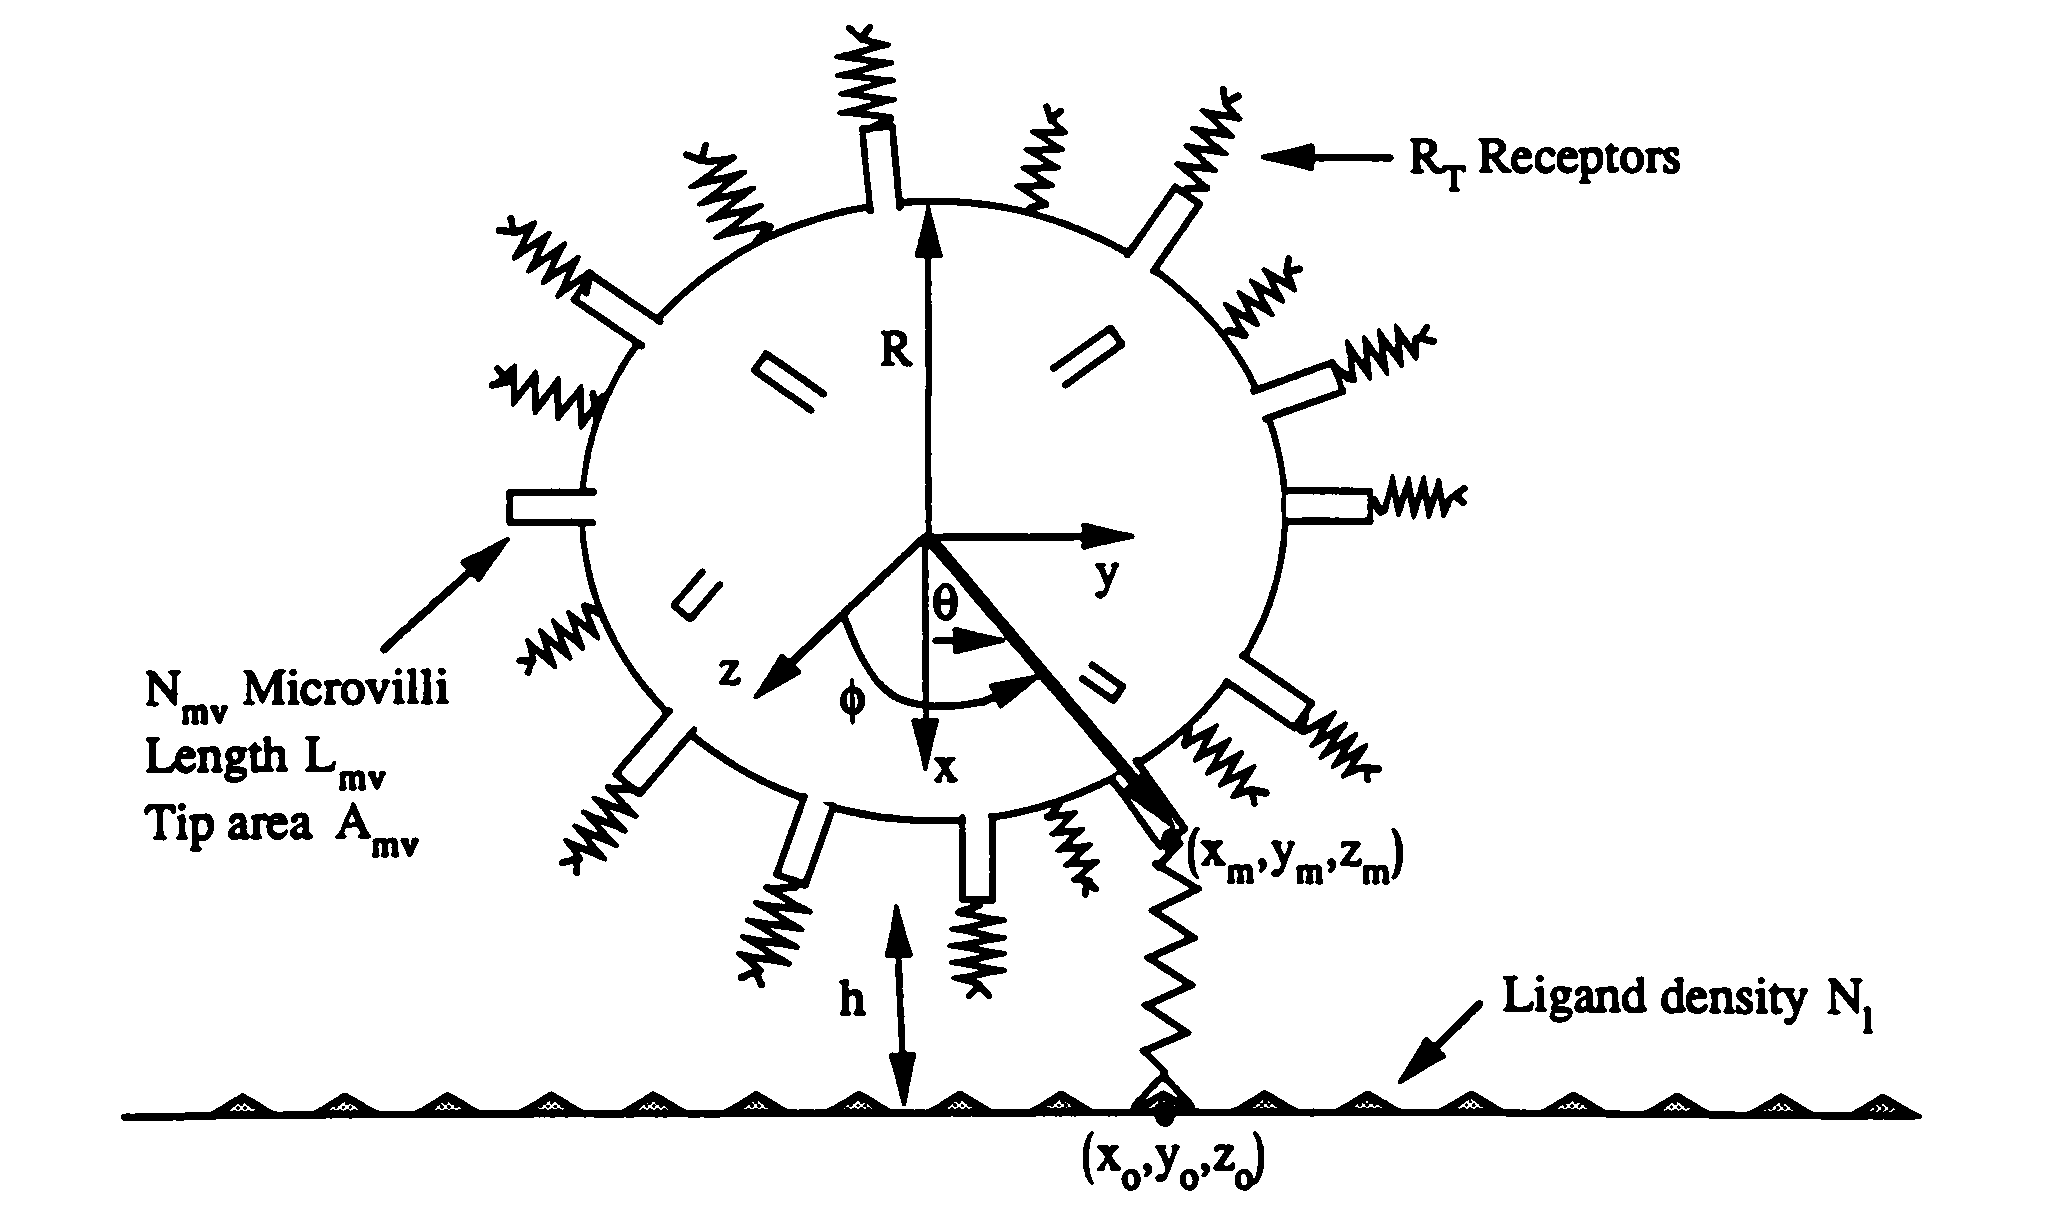
\includegraphics[width=\textwidth]{hammer92scr}}
      \caption{Geometry of a leukocyte AD model. From Hammer \&
        Apte, 1992}
      \label{fig:hammer-diagram}
    \end{figure}
  \end{column}
\end{columns}
\note[item] {We want to find parameters that give realistic rolling
  behavior in the 3D model, and tweak binding parameters to model the
  effects of priming on rolling behavior}
\end{frame}

\begin{frame}{Definitions and domain}
  \begin{columns}
    \begin{column}{.5\textwidth}
      \begin{itemize}
      \item Fluid domain is the upper half space where $x > 0$
      \item Wall is the plane at $x = 0$
      \item Background flow: $\vect{v}^\infty = \gamma x \vect{e}_z$
      \item Platelet: ellipsoid with axes $1.5 \times 1.5 \times 0.5$,
        center of mass at $\vect{x}_c$, orientation vector
        $\vect{e}_m$
        \note[item] {$\vect{e}_m$ is a unit vector in the direction of
          the minor axis. This is sufficient to define the
          orientation, since the platelet is rotationally symmetric
          about the minor axis} 
      \item Steady Stokes, no-slip BCs on the wall and platelet
        surface:
        \begin{align*}
          &\Delta \vect{v} = \nabla P, \, \nabla \cdot
            \vect{v} = 0 \\
          &\vect{v}(\vect{x})|_{\partial P} = \vect{U} +
            \vect{\Omega} \times \vect{x} \\
          &\vect{v}|_{x = 0} = 0, \, \vect{v}(\vect{x})|_{\|\vect{x}\|
            \rightarrow \infty} \rightarrow \vect{v}^\infty(\vect{x}) 
        \end{align*}
        \note[item] {$\vect{U}$ is the translational velocity of the
          platelet, and $\vect{\Omega}$ is the angular velocity of the
          platelet. Next, talk about platelet motion.}
      \end{itemize}
    \end{column}

    \begin{column}{.4\textwidth}
      \begin{figure}
        \centering
        \subfloat{\fbox{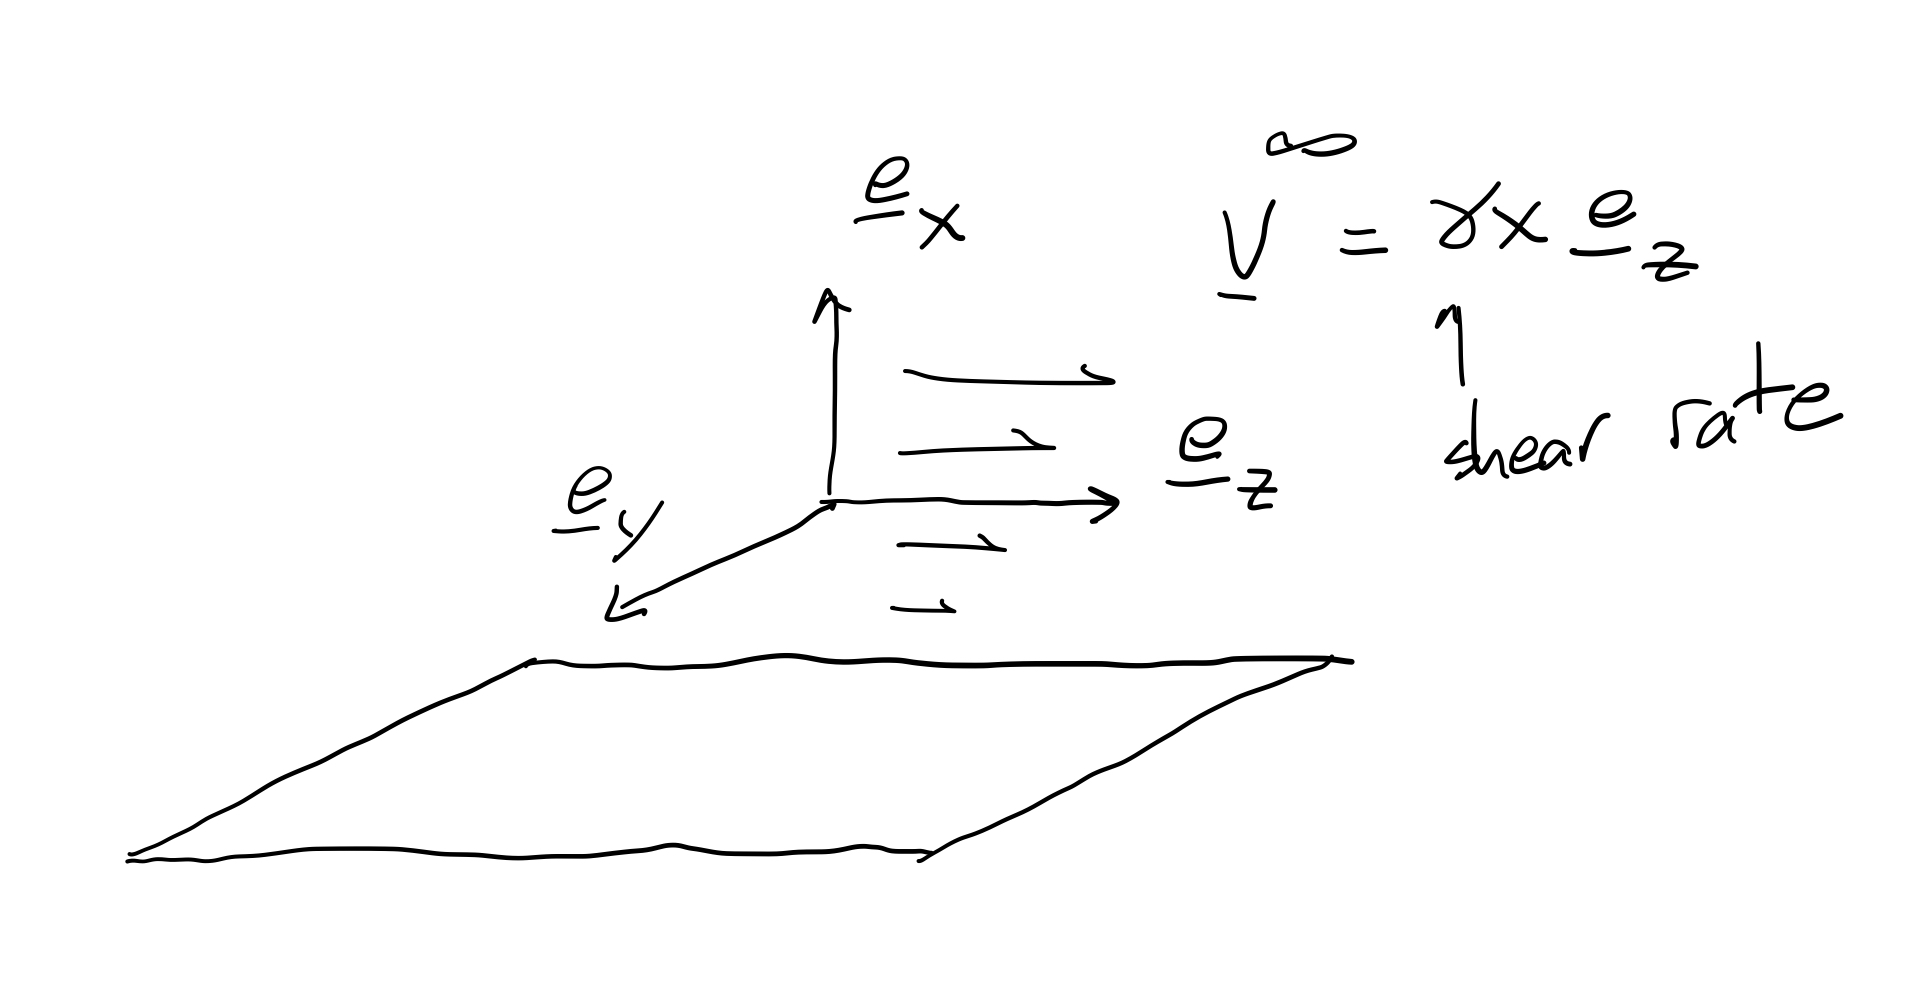
\includegraphics[width=\textwidth]{axes}}} \\
        \subfloat{\fbox{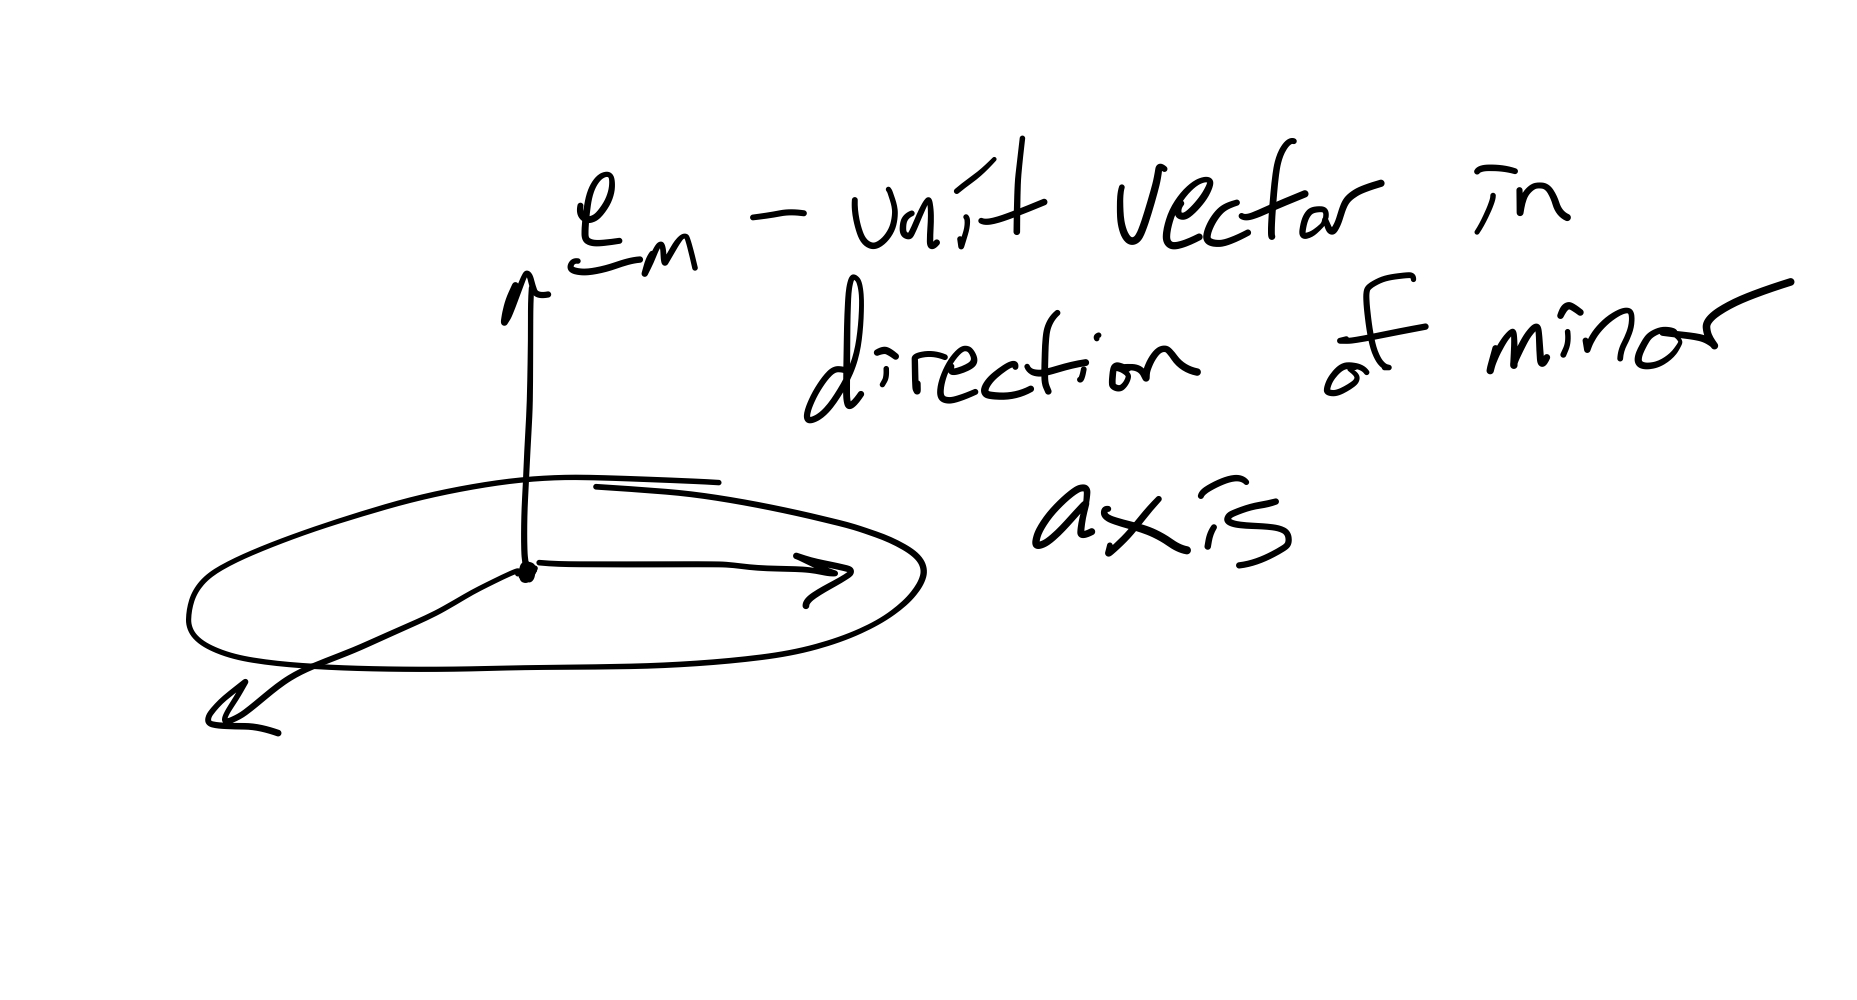
\includegraphics[width=\textwidth]{reference}}} 
        \caption{Sketch of the axes and orientation of the ellipsoid}
        \label{fig:orient-sketch}
      \end{figure}
    \end{column}
  \end{columns}
\end{frame}

\begin{frame}{Platelet motion}
  \begin{itemize}
  \item Equations of rigid body motion:
    \begin{equation*}
      \frac{d\vect{x}_c}{dt} = \vect{U}(\vect{x}_c, \vect{e}_m), \,
      \frac{d\vect{e}_m}{dt} = \vect{\Omega}(\vect{x}_c, \vect{e}_m)
      \times \vect{e}_m
    \end{equation*}
  \item $\vect{U}$ and $\vect{\Omega}$ are found by balancing forces
    and torques.
  \item Forces acting on the platelet:
    \begin{itemize}
    \item $\vect{F}^h$---hydrodynamic forces/torques
    \item $\vect{F}^o$---all other forces/torques
    \end{itemize}
    \note[item] {Most significantly bond forces, however past adhesive
      dynamics simulations have included other chemical forces acting
      on the platelet as well.}
  \item Given a velocity field $\vect{v}$ (and with
    $\underline{\underline{\sigma}} = -p \underline{\underline{I}} +
    \mu \left(\nabla \vect{v} + \left(\nabla \vect{v}\right)^T\right)$, then
    \begin{align*}
      \left[\vect{F}^h\right]_{1:3}
      &= \int_{\partial P} \underline{\underline{\sigma}} \cdot
        \vect{n} ds(\vect{x}) \\
      \left[\vect{F}^h\right]_{4:6}
      &= \int_{\partial P} (\vect{x} - \vect{x}_c) \times
        \underline{\underline{\sigma}} \cdot \vect{n} ds(\vect{x}) 
    \end{align*}
    \note[item] {$\sigma$ is the stress tensor of $\vect{v}$}
  \item If we assume $\vect{F}^o$ and $\vect{T}^o$ are known given a
    position and orientation, then we ``just'' need to find $\vect{U}$
    and $\vect{\Omega}$ such that $\vect{F}^h + \vect{F}^o = 0$
    \note[item] {This is hard because we need $\vect{U}$ and
      $\vect{\Omega}$ to solve Stokes' equations, but these are
      unknown at the start of a time step.}
  \end{itemize}
\end{frame}

\begin{frame}{Solving for $\vect{U}$ and $\vect{\Omega}$}
  \begin{itemize}
  \item Decompose $\vect{F}^h$:
    \begin{itemize}
    \item $\vect{F}^d$---drag force/torque on a moving platelet in a
      stationary flow 
    \item $\vect{F}^s$---drag force on a stationary platelet in a
      background shear flow 
    \end{itemize}
  \item Because of the linearity of Stokes flow, there is a linear
    relationship between $\vect{F}^d$ and $\vect{U}$: $\vect{F}^d =
    \underline{\underline{R}} \vect{U}$
  \item The resistance matrix depends only on the shape of the body, its
    position, and orientation
  \item To find $\underline{\underline{R}}$, solve 6 Stokes flow
    problems with BCs:
    \begin{align*}
      \vect{v}_i|_{\vect{x} \in \partial P}
      &= \delta_{ij} \vect{e}_j \tn{ for } i = 1, 2, 3 \tn{, and} \\
      \vect{v}_i|_{\partial P}
      &= \delta_{i-3, j} \vect{e}_j \times \vect{x} \tn{ for } i = 4,
        5, 6
    \end{align*}
  \item (with no-slip on the wall, and $\vect{v}_i \rightarrow
    \vect{0}$ as $\|\vect{x}\| \rightarrow \infty$)
  \item $\vect{F}^s$ is found with the 7th solve, with BCs
    $\vect{v}_7|_{\partial P} = \vect{0}$ and $\vect{v}_7 \rightarrow
    \gamma x \vect{e}_z$ as $\|x\| \rightarrow \infty$
  \end{itemize}
  \note[item] {Once these 7 velocity fields are formed, the $\vect{v}$
    generated by any rigid-body motion of the platelet can be found by
    taking the appropriate linear combination of $v_1$ through $v_7$,
    though we never actually do this. We only care about motion of the
    platelet.} 
\end{frame}

\begin{frame}{Model reproduces the two\footnote{There is a third type
      of motion, which occurs when the platelet is too far from the
      wall to make close contact} types of motion}
  % \begin{enumerate}
  % \item Pole-vaulting---when the platelet center of mass is between
  %   $\sim 1.0$--$1.5 \, \mu m$ from the wall
  % \item Surfing---when the platelet center of mass is $< 1.0 \, \mu m$
  %   from the wall (videos)
  % \end{enumerate}

  \begin{figure}
    \centering
    \includegraphics[width=.75\textwidth]{run18_fig}
    \caption{``Pole-vaulting''---when the platelet center of mass
      starts between $\sim 1.0$--$1.5 \, \mu m$ from the wall}
    \label{fig:free-rolling}
  \end{figure}
\end{frame}

\begin{frame}{Model reproduces the two types of motion}
  \begin{figure}
    \centering
    \includegraphics[width=.75\textwidth]{run56_fig}
    \caption{``Surfing''---when the platelet center of mass starts $<
      1.0 \, \mu m$ from the wall} 
    \label{fig:free-rolling}
  \end{figure}
\end{frame}

\begin{frame}{Model reproduces the two types of motion}
  Videos!
\end{frame}

\begin{frame}{Results from some binding experiments}
  % Parameters chosen fairly arbitrarily, but we can get good
  % estimates from the literature for the off rate, bond stiffness,
  % bond lengths

  % Simulations all start with the same initial condition: a flat
  % platelet at a height of 1.2 microns (so all platelets are in a
  % pole-vaulting regime initially)

  \begin{figure}
    \centering
    \parbox{0.49\textwidth}{
      \includegraphics[width=0.9\linewidth]{bd_runner1101_plot14.png}
    }
    \hfill
    \parbox{0.49\textwidth}{
      \includegraphics[width=0.9\linewidth]{bd_runner1103_plot2.png}
    }
    \caption{Sample trajectories at low (left) and high (right)
      on-rates.}
    % These plots are very messy. The solid lines in the upper plot
    % show the position of the platelet along the length of the flow
    % chamber. The bottom plot shows bond numbers over time
    \label{fig:sample-trajectories}
  \end{figure}
\end{frame}

\begin{frame}{Results from some binding experiments}
  % Parameters chosen fairly arbitrarily, but we can get good
  % estimates from the literature for the off rate, bond stiffness,
  % bond lengths

  % No good estimates for the on-rate
  \begin{figure}
    \centering
    \parbox{0.49\textwidth}{
      \includegraphics[width=\linewidth]{avel_avg_5.png}
    }
    \hfill
    \parbox{0.49\textwidth}{
      \includegraphics[width=\linewidth]{avg_vels_5.png}
    }
    \caption{Means of average velocities decrease with increasing
      on-rate, and histograms show bimodality}
    \label{fig:plot1}
  \end{figure}
\end{frame}

\begin{frame}{Results from some binding experiments}
  % Parameters chosen fairly arbitrarily, but we can get good
  % estimates from the literature for the off rate, bond stiffness,
  % bond lengths

  % No good estimates for the on-rate
  \begin{figure}
    \centering
    \parbox{0.49\textwidth}{
      \includegraphics[width=\linewidth]{dwell_avg_5.png}
    }
    \hfill
    \parbox{0.49\textwidth}{
      \includegraphics[width=\linewidth]{step_avg_5.png}
    }

    % Steps are not in the same ballpark as experimental (a few microns)
    \caption{Pause times increase with increasing on-rate (left), and step
      sizes decrease (right)}
    \label{fig:plot2}
  \end{figure}
\end{frame}

\begin{frame}{Bond lifetimes are exponentially distributed}
  \begin{figure}
    \centering
    \parbox{0.49\textwidth}{
      \includegraphics[width=\linewidth]{bdlf_8.png}
    }
    \hfill
    \parbox{0.49\textwidth}{
      \includegraphics[width=\linewidth]{steps_5.png}
    }
    \caption{Histograms of bond lifetimes and step sizes}
    \label{fig:lifetimes-and-steps}
  \end{figure}
\end{frame}

\begin{frame}{Other stuff}
  % Off rate, receptor number, randomized initial conditions
  \begin{itemize}
  \item Running other experiments testing changes in other parameters:
    off rate, number of receptors, randomized intial platelet heights
    (picked from distribution estimates from whole blood experiments)
  \item Fixing/Checking some data extraction stuff
  \item Reviewing literature estimates of binding parameters
    ($k_\text{on}$ in particular)
  \end{itemize}
\end{frame}

\end{document}
